% Klokan program documentation, 24/05/2017, Jan Horesovsky
\documentclass{article}
\usepackage[utf8]{inputenc}
\usepackage[T1]{fontenc}
\usepackage[english,czech]{babel}
\usepackage{parskip}
\selectlanguage{english}

\usepackage{amsmath}
\usepackage{graphicx}

\begin{document}
\title{Klokan - Program Documentation}
\author{Jan Horešovský}
\date{May 2017}
\pagenumbering{gobble}
\maketitle

Klokan is a program which can be used to evaluate Mathematical Kangaroo answer sheets.

\section{User Documentation}{
Klokan is a console program which is made for launching from the command line. It takes unedited \verb+.jpg+ scans of an answer sheet containing correct answers and answer sheets to be evaluated. After the program finishes, text files containing its output can be found in the current folder. The process of evaluating answer sheets can be parameterized using a configuration file.
	
	\subsection{Input}{
	Paths to scans are given to the program in the form of command-line arguments. Each path has to be separated by a space.
	\begin{itemize}
		\item The first argument is the path to the answer sheet containing correct answers.
		\item All the other arguments are paths to answer sheets to be evaluated.
	\end{itemize}
	}

	\subsection{Output}{
	For each answer sheet that the program evaluates, one text file containing the results of the evaluation is generated. If the original answer sheet is called \verb+sheet.jpg+, then the output file will be called \verb+sheetRESULT.txt+.

	On top of that, the program outputs informative and error messages to the standard error output which is displayed in the command line.

	\subsection{Configuration File}
	This section is only for advanced users!

	The configuration file can be used to tweak the evaluation process by changing some parameters. It has to be called \verb+config.txt+ and placed in the program folder. Each parameter has to be on a separate line, no empty lines are allowed and the order of the parameters can be arbitrary. Here is the format of a line:
	\begin{center}
	{\it parameter\_name}={\it parameter\_value} \par
	\end{center}
	
	For example:
	\begin{center}
	default\_sheet\_width=1700 \par
	\end{center}
	}

		\subsubsection{Parameter Description}{
			\begin{description}
				\item [default\_sheet\_width] [{\it integer value (500-5000)}] This parameter determines the width to which every sheet will be resized before processing while preserving the original aspect ratio. This influences line recognition since a line in a high resolution image will have more pixels.
				\item [black\_white\_threshold] [{\it integer value (0-255)}] This parameter influences the conversion of the sheet to a binary image. All pixels up to this value will be recognized as black and all the others as white. Useful for recognizing or ignoring very light lines made with a pencil for example.
				\item [table\_line\_length] [{\it integer value}] This parameter says how long a line has to be in order to be recognized as a border line of a table. Has to be set depending on \verb+default_sheet_width+.
				\item [table\_line\_eccentricity\_limit] [{\it floating-point value in radians (0-$\pi / 4$)}] This parameter determines how slanted a table line can be in order to still be recognized as vertical or horizontal. Can be tweaked if very slanted scans need to be recognized. Can break the recognition process if set too high.
				\item [table\_line\_curvature\_limit] [{\it integer value (1-)}] This parameter says how curved a table line can be in order to be recognized as straight.
				\item [default\_cell\_width] [{\it integer value (10-500)}] See \verb+default_sheet_width+, used for cells.
				\item [default\_cell\_height] [{\it integer value (10-500)}] See \verb+default_sheet_width+, used for cells.
				\item [cross\_line\_length] [{\it integer value}] This parameter says how long a line in a cell has to be in order to be recognized as a potential cross line. Has to be set depending on the dimensions of the cell.
				\item [cross\_line\_curvature\_limit] [{\it integer value (1-)}] This parameter says how curved a cell line can be in order to be recognized as straight.
				\item [rubbish\_lines\_limit] [{\it integer value}] This parameter determines how many non-diagonal lines in a cell should be ignored as noise. If a cell has more non-diagonal lines than that, it is automatically considered not crossed.
			\end{description}
		}
	
}

\section{Developer Documentation}{
This section thoroughly describes the architecture of Klokan and also mentions one implementation detail which is mathematically more challenging and might not be clear from the source code.
	\subsection{Overview}{
	The program is based on deterministic image recognition using simple geometric algorithms. These, and also some other functionality necessary for image processing is taken from the OpenCV library version 3.1.0. The whole program is written in C++. It basically provides two kinds of functionality. First, it has interface functions which do the image recognition itself and are able to tell which answers have been chosen. When the program is compiled as a \verb+.dll+ these can be used to create a custom evaluation program with a specific user interface and input and output mechanisms. Next to this, Klokan also provides a very simple implementation of the evaluation program - a command-line user interface with input in the form of program arguments and output in the form of text files.
	
	The process of evaluating an answer sheet comprises three stages:
	\begin{itemize}
		\item Table Extraction
		\item Cell Extraction
		\item Cell Evaluation
	\end{itemize}

	These also correspond to the three interface functions that this program provides. The program logic is implemented in the \verb+Klokan+ class. Parameters of image recognition can be set using a configuration file or they can be left at their default value.

		\subsubsection{Table Extraction}{
		Some preprocessing steps have to be made before the answer sheet is processed. First, the width of the sheet is changed (\verb+default_sheet_width+ parameter) while preserving the original aspect ratio. After that the sheet is thresholded and converted to binary (\verb+black_white_threshold+) and then inverted.

		\begin{center}
			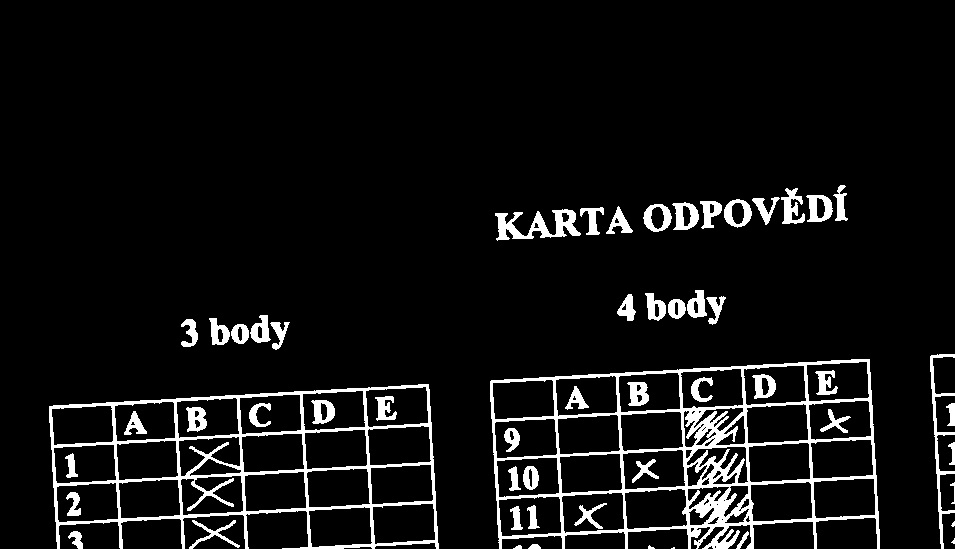
\includegraphics[width=10cm]{01.jpg} \par
			{\bf Fig. 1} Thresholded and inverted image. \par
		\end{center}

		In order to extract tables from the answer sheet the program needs to find them first. Tables are generally the largest objects in the sheet, so instead of looking for tables the program simply looks for the largest object. This is done by using an OpenCV function \verb+flood_fill()+. This function takes a pixel and floods it and all its neighbouring pixels (and all their neighbouting pixels...) which have the same colour as the starting pixel. Then it returns a number which represents the area which has been flooded. This way the program finds out where the upper left pixel of the largest object is. When this table is extracted, it is hidden (flooded with black) and the second largest object (another table) is found.

		\begin{center}
			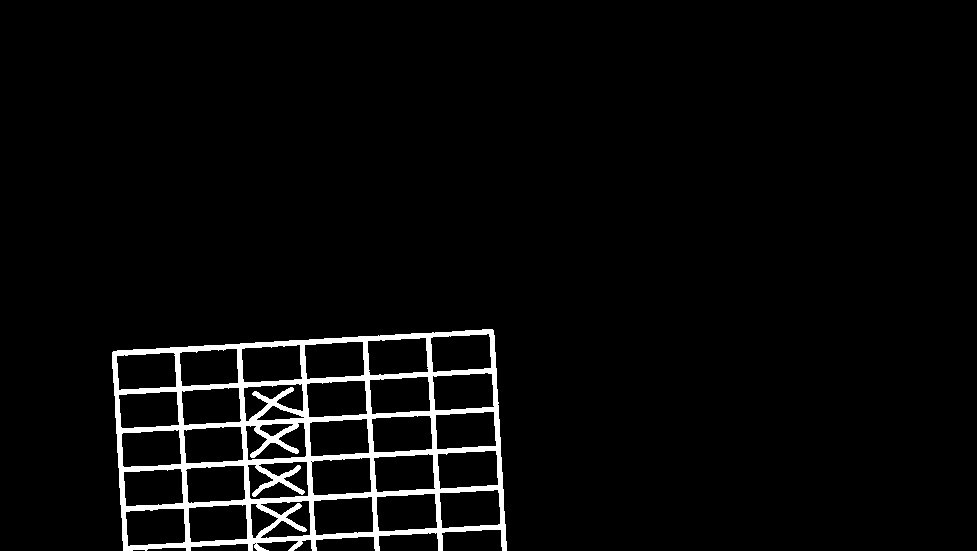
\includegraphics[width=10cm]{02.jpg} \par
			{\bf Fig. 2} A table is found and the rest of the image hidden. \par
		\end{center}

		After the program finds a table, it creates a copy of the sheet in which it hides all other parts of the image. Then it uses an OpenCV function called \verb+hough_lines()+ to find all the lines in the table. The function is set so that it only finds lines that are at least as long as the expected edge of the table (\verb+table_line_length+, \verb+table_line_curvature_limit+). These lines also need to be only almost horizontal or almost vertical (\verb+table_line_eccentricity_limit+) because they are expected to form a rectangular table. After that the corners of the table are found by taking the extreme lines and their intersections.

		\begin{center}
			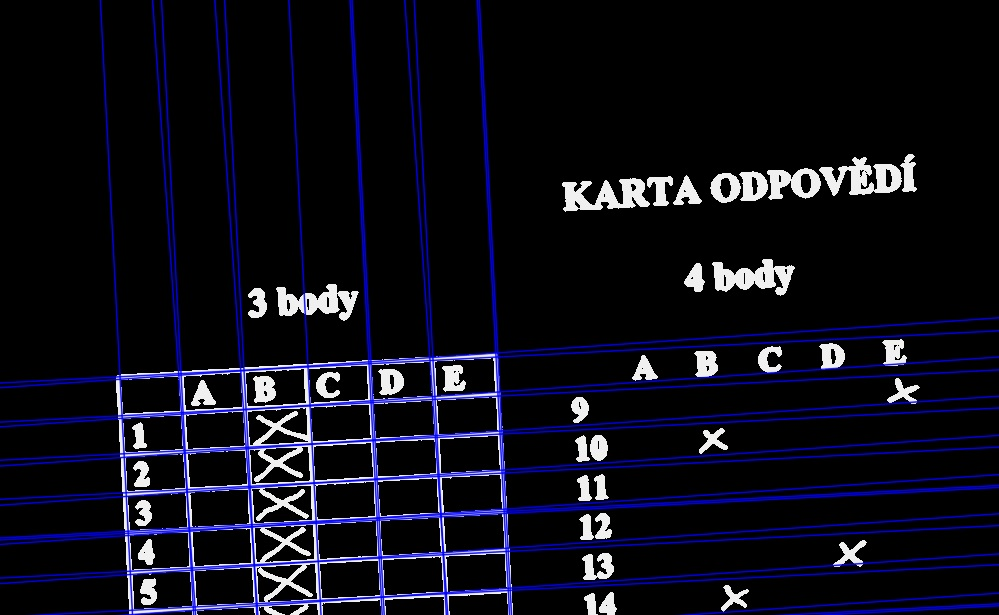
\includegraphics[width=10cm]{04.jpg} \par
			{\bf Fig. 3} Table lines found. \par
		\end{center}

		\begin{center}
			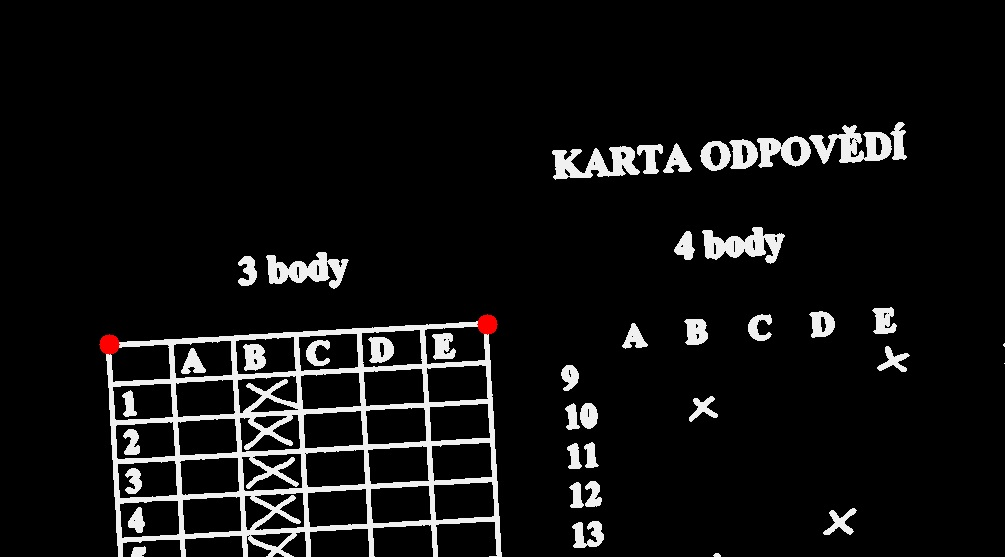
\includegraphics[width=10cm]{03.jpg} \par
			{\bf Fig. 4} Corners of the table found. \par
		\end{center}

		The table does not generally have to be perfectly aligned with the edges of the image. However, this is taken care of by using the corner points and an OpenCV function called \verb+crop_perspective()+ which maps these corner points onto the corner points of a square. This square has a side equal to the edge of the table. After that other points are transformed accordingly and the program obtains a new image containing only the table which is now perfectly aligned. This step is important for being able to cut the table into cells easily.
		}

		\subsubsection{Cell Extraction}{
		When a table is extracted and aligned, it is easy to cut it into cells based on the number of rows and columns which for the standard Mathematical Kangaroo answer sheet is 9 and 6 respectively.

		\begin{center}
			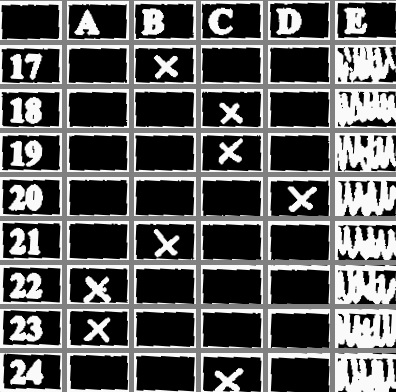
\includegraphics[width=5cm]{05.jpg} \par
			{\bf Fig. 5} Table is aligned and split into cells. \par
		\end{center}
		}

		\subsubsection{Cell Evaluation}{
		Each cell is then evaluated using the function \verb+is_cell_crossed()+ which simply returns \verb+true+ or \verb+false+.

		The dimensions of the cell are changed first (\verb+default_cell_...+ arguments). After that all lines in the cell are detected (\verb+cross_line_...+ arguments) and split into three groups: left-up-bottom-right, right-up-bottom-left and other. If a cell contains at least one line from the first two groups and not too many other lines (\verb+rubbish_lines_limit+), it is crossed. Otherwise, it is not.
		}

		\subsubsection{Klokan}{
		One run of the program corresponds to one batch of answer sheets taken from the program arguments. This is taken care of in the \verb+run()+ function of the \verb+Klokan+ class. It accepts the name of the sheet with correct answers and then the names of all the other answer sheets which are to be evaluated. First, it extracts the answers from the correct answer sheet and saves them for future reference. After that it evaluates the other answer sheets in a loop where it does three things:
		\begin{itemize}
			\item it finds all mistakes and corrects them resulting in a new data structure containing all the answers including the wrong ones and the corrected ones
			\item it uses this data structure to count the score based on the standard rules of the Mathematical Kangaroo
			\item it outputs a file containing all answers including the corrected and wrong ones and the score
		\end{itemize}

		After the \verb+run()+ function returns, the program ends.
		}

		\subsubsection{Configuration File}{
		The configuration file is loaded at the beginning of the program. The default value of each parameter mentioned in the file is rewritten. If there is any error in the configuration file, the loading process is stopped and default values are used for all parameters that have not been rewritten up to this point.
		}
	}

	\subsection{Implementation Details}{
		\subsubsection{Intersection Between Two Lines}{
		In the function \verb+find_intersection()+ in file \verb+table_extract.cpp+, an intersection between two lines needs to be found in order to determine a corner of a table. First thing to note the representation of lines in OpenCV.

		Each line in OpenCV is represented by two floating-point numbers: $\rho$ and $\theta$. $\rho$ represents the perpendicular distance from the origin to the line and $\theta$ is the angle by which you have to rotate the $(\rho, 0)$ vector in order to get that perpendicular distance. This is true if the line passes below the origin. If it passes above the origin, the situation is the same, except $\rho$ is taken negative, so that $\theta$ can be less that $180^\circ$.

		This means that the line can be described like this:
		\begin{align*}
			a \cdot x + b \cdot y + c &= 0 \\
			\cos \theta \cdot x + \sin \theta \cdot y - \rho &= 0
		\end{align*}

		Now we can use homogenous coordinates to find the intersection:
		\begin{align*}
			P &= U_1 \times U_2 \\
			(a_p, b_p, c_p) &= (a_1, b_1, c_1) \times (a_2, b_2, c_2) \\
			(a_p, b_p, c_p) &= (\cos \theta_1, \sin \theta_1, -\rho_1) \times (\cos \theta_2, \sin \theta_2, -\rho_2)
		\end{align*}
		where $P$ is the intersection and $U_1 \times U_2$ is the cross product of the homogenous coordinates of the lines. In order to get the Euclidean coordinates of $P$, we simply take
		\begin{align*}
			P'_x &= a_p / c_p \\
			P'_y &= b_p / c_p
		\end{align*}
		}
	}
}

\end{document}
